\documentclass[1p]{elsarticle_modified}
%\bibliographystyle{elsarticle-num}

%\usepackage[colorlinks]{hyperref}
%\usepackage{abbrmath_seonhwa} %\Abb, \Ascr, \Acal ,\Abf, \Afrak
\usepackage{amsfonts}
\usepackage{amssymb}
\usepackage{amsmath}
\usepackage{amsthm}
\usepackage{scalefnt}
\usepackage{amsbsy}
\usepackage{kotex}
\usepackage{caption}
\usepackage{subfig}
\usepackage{color}
\usepackage{graphicx}
\usepackage{xcolor} %% white, black, red, green, blue, cyan, magenta, yellow
\usepackage{float}
\usepackage{setspace}
\usepackage{hyperref}

\usepackage{tikz}
\usetikzlibrary{arrows}

\usepackage{multirow}
\usepackage{array} % fixed length table
\usepackage{hhline}

%%%%%%%%%%%%%%%%%%%%%
\makeatletter
\renewcommand*\env@matrix[1][\arraystretch]{%
	\edef\arraystretch{#1}%
	\hskip -\arraycolsep
	\let\@ifnextchar\new@ifnextchar
	\array{*\c@MaxMatrixCols c}}
\makeatother %https://tex.stackexchange.com/questions/14071/how-can-i-increase-the-line-spacing-in-a-matrix
%%%%%%%%%%%%%%%

\usepackage[normalem]{ulem}

\newcommand{\msout}[1]{\ifmmode\text{\sout{\ensuremath{#1}}}\else\sout{#1}\fi}
%SOURCE: \msout is \stkout macro in https://tex.stackexchange.com/questions/20609/strikeout-in-math-mode

\newcommand{\cancel}[1]{
	\ifmmode
	{\color{red}\msout{#1}}
	\else
	{\color{red}\sout{#1}}
	\fi
}

\newcommand{\add}[1]{
	{\color{blue}\uwave{#1}}
}

\newcommand{\replace}[2]{
	\ifmmode
	{\color{red}\msout{#1}}{\color{blue}\uwave{#2}}
	\else
	{\color{red}\sout{#1}}{\color{blue}\uwave{#2}}
	\fi
}

\newcommand{\Sol}{\mathcal{S}} %segment
\newcommand{\D}{D} %diagram
\newcommand{\A}{\mathcal{A}} %arc


%%%%%%%%%%%%%%%%%%%%%%%%%%%%%5 test

\def\sl{\operatorname{\textup{SL}}(2,\Cbb)}
\def\psl{\operatorname{\textup{PSL}}(2,\Cbb)}
\def\quan{\mkern 1mu \triangleright \mkern 1mu}

\theoremstyle{definition}
\newtheorem{thm}{Theorem}[section]
\newtheorem{prop}[thm]{Proposition}
\newtheorem{lem}[thm]{Lemma}
\newtheorem{ques}[thm]{Question}
\newtheorem{cor}[thm]{Corollary}
\newtheorem{defn}[thm]{Definition}
\newtheorem{exam}[thm]{Example}
\newtheorem{rmk}[thm]{Remark}
\newtheorem{alg}[thm]{Algorithm}

\newcommand{\I}{\sqrt{-1}}
\begin{document}

%\begin{frontmatter}
%
%\title{Boundary parabolic representations of knots up to 8 crossings}
%
%%% Group authors per affiliation:
%\author{Yunhi Cho} 
%\address{Department of Mathematics, University of Seoul, Seoul, Korea}
%\ead{yhcho@uos.ac.kr}
%
%
%\author{Seonhwa Kim} %\fnref{s_kim}}
%\address{Center for Geometry and Physics, Institute for Basic Science, Pohang, 37673, Korea}
%\ead{ryeona17@ibs.re.kr}
%
%\author{Hyuk Kim}
%\address{Department of Mathematical Sciences, Seoul National University, Seoul 08826, Korea}
%\ead{hyukkim@snu.ac.kr}
%
%\author{Seokbeom Yoon}
%\address{Department of Mathematical Sciences, Seoul National University, Seoul, 08826,  Korea}
%\ead{sbyoon15@snu.ac.kr}
%
%\begin{abstract}
%We find all boundary parabolic representation of knots up to 8 crossings.
%
%\end{abstract}
%\begin{keyword}
%    \MSC[2010] 57M25 
%\end{keyword}
%
%\end{frontmatter}

%\linenumbers
%\tableofcontents
%
\newcommand\colored[1]{\textcolor{white}{\rule[-0.35ex]{0.8em}{1.4ex}}\kern-0.8em\color{red} #1}%
%\newcommand\colored[1]{\textcolor{white}{ #1}\kern-2.17ex	\textcolor{white}{ #1}\kern-1.81ex	\textcolor{white}{ #1}\kern-2.15ex\color{red}#1	}

{\Large $\underline{11a_{227}~(K11a_{227})}$}

\setlength{\tabcolsep}{10pt}
\renewcommand{\arraystretch}{1.6}
\vspace{1cm}\begin{tabular}{m{100pt}>{\centering\arraybackslash}m{274pt}}
\multirow{5}{120pt}{
	\centering
	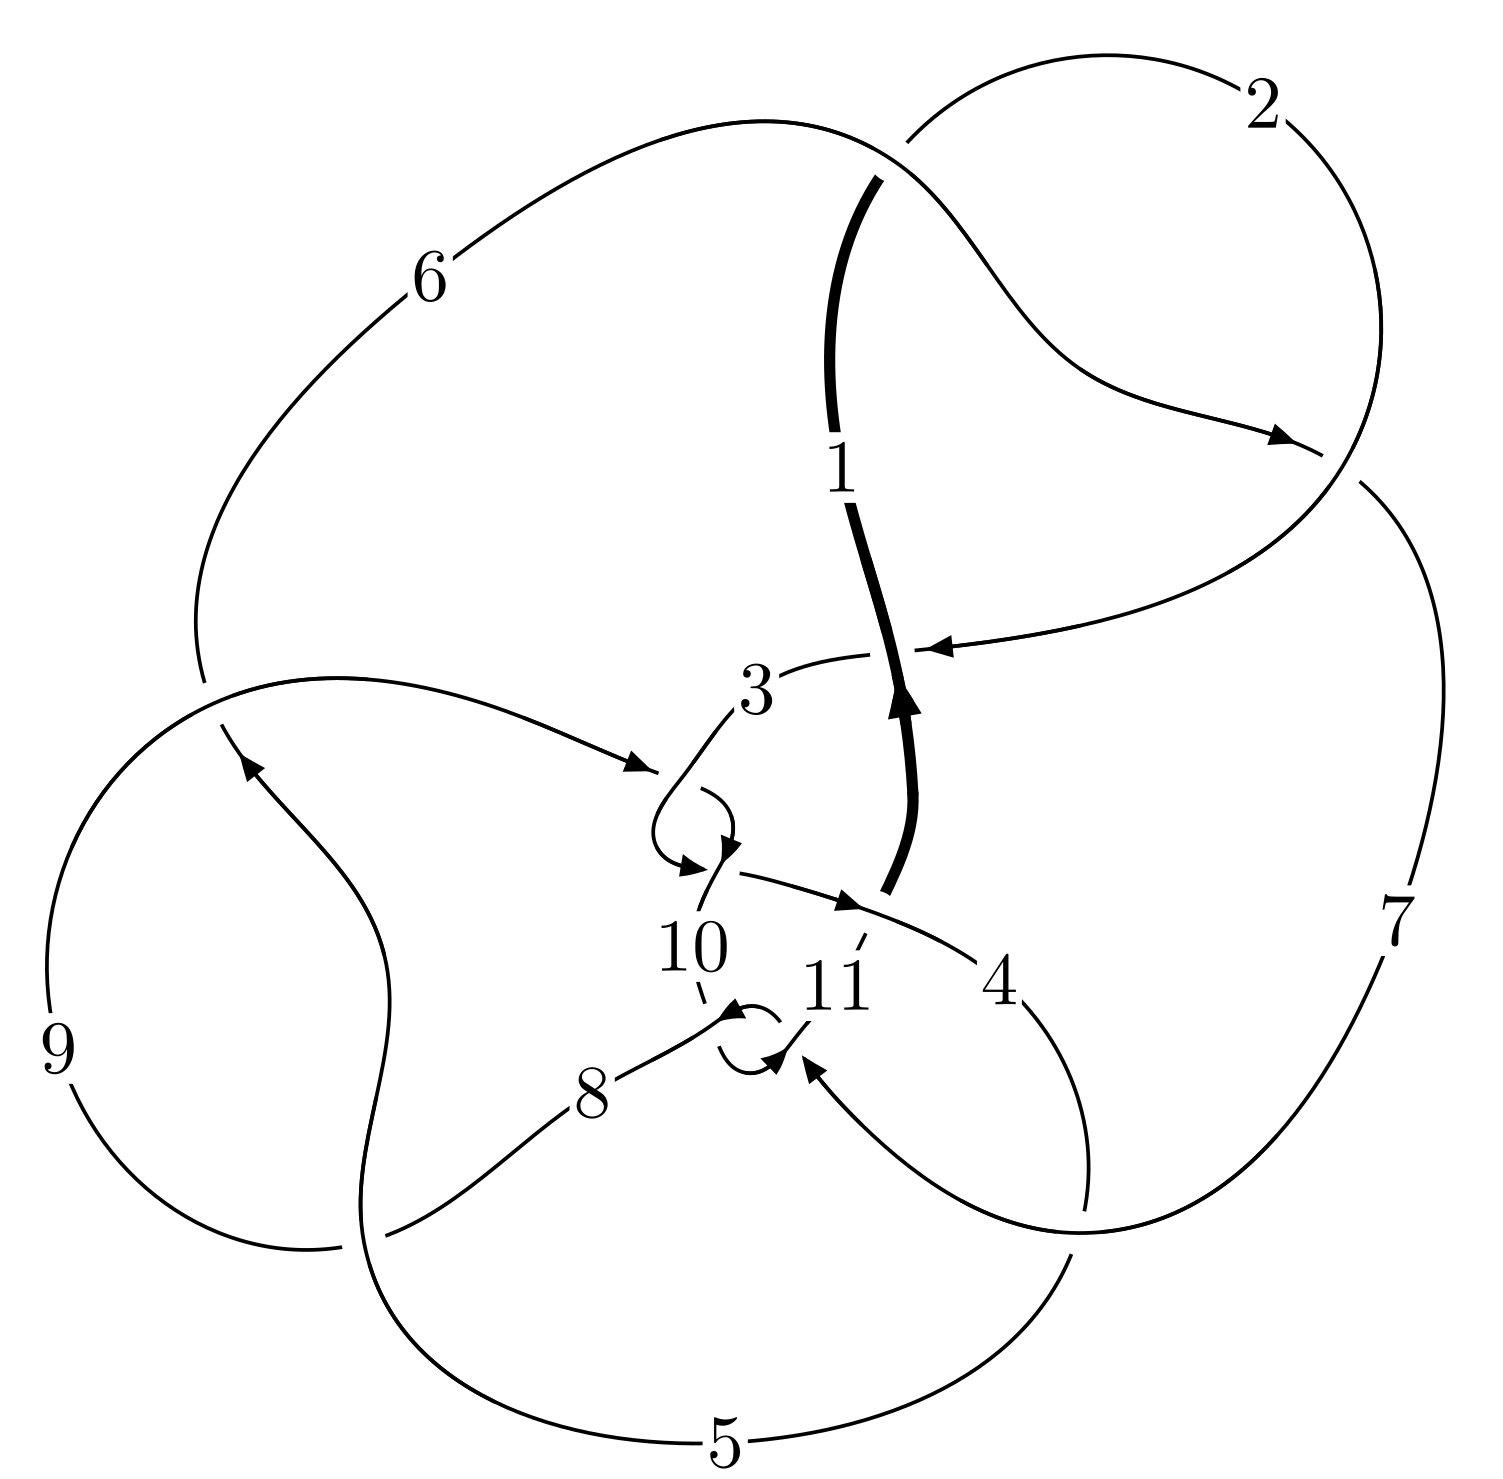
\includegraphics[width=112pt]{../../../GIT/diagram.site/Diagrams/png/476_11a_227.png}\\
\ \ \ A knot diagram\footnotemark}&
\allowdisplaybreaks
\textbf{Linearized knot diagam} \\
\cline{2-2}
 &
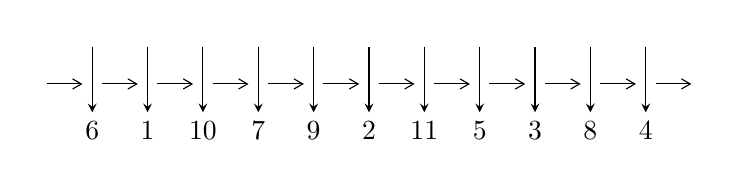
\begin{tikzpicture}[x=20pt, y=17pt]
	% nodes
	\node (C0) at (0, 0) {};
	\node (C1) at (1, 0) {};
	\node (C1U) at (1, +1) {};
	\node (C1D) at (1, -1) {6};

	\node (C2) at (2, 0) {};
	\node (C2U) at (2, +1) {};
	\node (C2D) at (2, -1) {1};

	\node (C3) at (3, 0) {};
	\node (C3U) at (3, +1) {};
	\node (C3D) at (3, -1) {10};

	\node (C4) at (4, 0) {};
	\node (C4U) at (4, +1) {};
	\node (C4D) at (4, -1) {7};

	\node (C5) at (5, 0) {};
	\node (C5U) at (5, +1) {};
	\node (C5D) at (5, -1) {9};

	\node (C6) at (6, 0) {};
	\node (C6U) at (6, +1) {};
	\node (C6D) at (6, -1) {2};

	\node (C7) at (7, 0) {};
	\node (C7U) at (7, +1) {};
	\node (C7D) at (7, -1) {11};

	\node (C8) at (8, 0) {};
	\node (C8U) at (8, +1) {};
	\node (C8D) at (8, -1) {5};

	\node (C9) at (9, 0) {};
	\node (C9U) at (9, +1) {};
	\node (C9D) at (9, -1) {3};

	\node (C10) at (10, 0) {};
	\node (C10U) at (10, +1) {};
	\node (C10D) at (10, -1) {8};

	\node (C11) at (11, 0) {};
	\node (C11U) at (11, +1) {};
	\node (C11D) at (11, -1) {4};
	\node (C12) at (12, 0) {};

	% arrows
	\draw[->,>={angle 60}]
	(C0) edge (C1) (C1) edge (C2) (C2) edge (C3) (C3) edge (C4) (C4) edge (C5) (C5) edge (C6) (C6) edge (C7) (C7) edge (C8) (C8) edge (C9) (C9) edge (C10) (C10) edge (C11) (C11) edge (C12) ;	\draw[->,>=stealth]
	(C1U) edge (C1D) (C2U) edge (C2D) (C3U) edge (C3D) (C4U) edge (C4D) (C5U) edge (C5D) (C6U) edge (C6D) (C7U) edge (C7D) (C8U) edge (C8D) (C9U) edge (C9D) (C10U) edge (C10D) (C11U) edge (C11D) ;
	\end{tikzpicture} \\
\hhline{~~} \\& 
\textbf{Solving Sequence} \\ \cline{2-2} 
 &
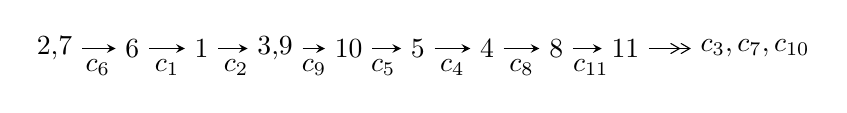
\begin{tikzpicture}[x=25pt, y=7pt]
	% node
	\node (A0) at (-1/8, 0) {2,7};
	\node (A1) at (1, 0) {6};
	\node (A2) at (2, 0) {1};
	\node (A3) at (49/16, 0) {3,9};
	\node (A4) at (33/8, 0) {10};
	\node (A5) at (41/8, 0) {5};
	\node (A6) at (49/8, 0) {4};
	\node (A7) at (57/8, 0) {8};
	\node (A8) at (65/8, 0) {11};
	\node (C1) at (1/2, -1) {$c_{6}$};
	\node (C2) at (3/2, -1) {$c_{1}$};
	\node (C3) at (5/2, -1) {$c_{2}$};
	\node (C4) at (29/8, -1) {$c_{9}$};
	\node (C5) at (37/8, -1) {$c_{5}$};
	\node (C6) at (45/8, -1) {$c_{4}$};
	\node (C7) at (53/8, -1) {$c_{8}$};
	\node (C8) at (61/8, -1) {$c_{11}$};
	\node (A9) at (10, 0) {$c_{3},c_{7},c_{10}$};

	% edge
	\draw[->,>=stealth]	
	(A0) edge (A1) (A1) edge (A2) (A2) edge (A3) (A3) edge (A4) (A4) edge (A5) (A5) edge (A6) (A6) edge (A7) (A7) edge (A8) ;
	\draw[->>,>={angle 60}]	
	(A8) edge (A9);
\end{tikzpicture} \\ 

\end{tabular} \\

\footnotetext{
The image of knot diagram is generated by the software ``\textbf{Draw programme}" developed by Andrew Bartholomew(\url{http://www.layer8.co.uk/maths/draw/index.htm\#Running-draw}), where we modified some parts for our purpose(\url{https://github.com/CATsTAILs/LinksPainter}).
}\phantom \\ \newline 
\centering \textbf{Ideals for irreducible components\footnotemark of $X_{\text{par}}$} 
 
\begin{align*}
I^u_{1}&=\langle 
11 u^{29}-82 u^{28}+\cdots+4 b-92,\;527 u^{29}-5269 u^{28}+\cdots+32 a+9872,\;u^{30}-11 u^{29}+\cdots+192 u-32\rangle \\
I^u_{2}&=\langle 
11652760173 a^9 u^5+89806445727 a^8 u^5+\cdots+133817291376 a+47860828523,\\
\phantom{I^u_{2}}&\phantom{= \langle  }2 a^8 u^5-21 a^7 u^5+\cdots-94 a-49,\;u^6+u^5- u^4-2 u^3+u+1\rangle \\
I^u_{3}&=\langle 
u^{18}-2 u^{17}+\cdots+b-5,\;-5 u^{18}+u^{17}+\cdots+a+5,\;u^{19}-6 u^{17}+\cdots-3 u-1\rangle \\
\\
\end{align*}
\raggedright * 3 irreducible components of $\dim_{\mathbb{C}}=0$, with total 109 representations.\\
\footnotetext{All coefficients of polynomials are rational numbers. But the coefficients are sometimes approximated in decimal forms when there is not enough margin.}
\newpage
\renewcommand{\arraystretch}{1}
\centering \section*{I. $I^u_{1}= \langle 11 u^{29}-82 u^{28}+\cdots+4 b-92,\;527 u^{29}-5269 u^{28}+\cdots+32 a+9872,\;u^{30}-11 u^{29}+\cdots+192 u-32 \rangle$}
\flushleft \textbf{(i) Arc colorings}\\
\begin{tabular}{m{7pt} m{180pt} m{7pt} m{180pt} }
\flushright $a_{2}=$&$\begin{pmatrix}0\\u\end{pmatrix}$ \\
\flushright $a_{7}=$&$\begin{pmatrix}1\\0\end{pmatrix}$ \\
\flushright $a_{6}=$&$\begin{pmatrix}1\\- u^2\end{pmatrix}$ \\
\flushright $a_{1}=$&$\begin{pmatrix}u\\- u^3+u\end{pmatrix}$ \\
\flushright $a_{3}=$&$\begin{pmatrix}- u^3\\u^5- u^3+u\end{pmatrix}$ \\
\flushright $a_{9}=$&$\begin{pmatrix}-\frac{527}{32} u^{29}+\frac{5269}{32} u^{28}+\cdots+1810 u-\frac{617}{2}\\-\frac{11}{4} u^{29}+\frac{41}{2} u^{28}+\cdots-\frac{141}{2} u+23\end{pmatrix}$ \\
\flushright $a_{10}=$&$\begin{pmatrix}\frac{817}{32} u^{29}-\frac{8075}{32} u^{28}+\cdots-3086 u+\frac{1095}{2}\\\frac{11}{4} u^{29}-\frac{51}{4} u^{28}+\cdots+\frac{2501}{2} u-297\end{pmatrix}$ \\
\flushright $a_{5}=$&$\begin{pmatrix}\frac{293}{32} u^{29}-\frac{2921}{32} u^{28}+\cdots-1146 u+208\\-\frac{45}{16} u^{29}+\frac{529}{16} u^{28}+\cdots+840 u-167\end{pmatrix}$ \\
\flushright $a_{4}=$&$\begin{pmatrix}\frac{203}{32} u^{29}-\frac{1863}{32} u^{28}+\cdots-306 u+41\\-\frac{45}{16} u^{29}+\frac{529}{16} u^{28}+\cdots+840 u-167\end{pmatrix}$ \\
\flushright $a_{8}=$&$\begin{pmatrix}-34.7500 u^{29}+340.063 u^{28}+\cdots+3656.25 u-618.500\\\frac{41}{16} u^{29}-\frac{545}{16} u^{28}+\cdots-\frac{2761}{2} u+306\end{pmatrix}$ \\
\flushright $a_{11}=$&$\begin{pmatrix}-\frac{161}{32} u^{29}+\frac{1303}{32} u^{28}+\cdots-\frac{405}{2} u+74\\\frac{43}{4} u^{29}-\frac{877}{8} u^{28}+\cdots-1606 u+307\end{pmatrix}$\\ \flushright $a_{11}=$&$\begin{pmatrix}-\frac{161}{32} u^{29}+\frac{1303}{32} u^{28}+\cdots-\frac{405}{2} u+74\\\frac{43}{4} u^{29}-\frac{877}{8} u^{28}+\cdots-1606 u+307\end{pmatrix}$\\&\end{tabular}
\flushleft \textbf{(ii) Obstruction class $= -1$}\\~\\
\flushleft \textbf{(iii) Cusp Shapes $= \frac{125}{4} u^{29}-\frac{1153}{4} u^{28}+\cdots-1098 u+74$}\\~\\
\newpage\renewcommand{\arraystretch}{1}
\flushleft \textbf{(iv) u-Polynomials at the component}\newline \\
\begin{tabular}{m{50pt}|m{274pt}}
Crossings & \hspace{64pt}u-Polynomials at each crossing \\
\hline $$\begin{aligned}c_{1},c_{6}\end{aligned}$$&$\begin{aligned}
&u^{30}-11 u^{29}+\cdots+192 u-32
\end{aligned}$\\
\hline $$\begin{aligned}c_{2}\end{aligned}$$&$\begin{aligned}
&u^{30}+15 u^{29}+\cdots+6656 u+1024
\end{aligned}$\\
\hline $$\begin{aligned}c_{3},c_{5},c_{8}\\c_{9}\end{aligned}$$&$\begin{aligned}
&u^{30}+u^{29}+\cdots-4 u-1
\end{aligned}$\\
\hline $$\begin{aligned}c_{4},c_{11}\end{aligned}$$&$\begin{aligned}
&u^{30}- u^{29}+\cdots+5 u-1
\end{aligned}$\\
\hline $$\begin{aligned}c_{7},c_{10}\end{aligned}$$&$\begin{aligned}
&u^{30}-15 u^{29}+\cdots-608 u+64
\end{aligned}$\\
\hline
\end{tabular}\\~\\
\newpage\renewcommand{\arraystretch}{1}
\flushleft \textbf{(v) Riley Polynomials at the component}\newline \\
\begin{tabular}{m{50pt}|m{274pt}}
Crossings & \hspace{64pt}Riley Polynomials at each crossing \\
\hline $$\begin{aligned}c_{1},c_{6}\end{aligned}$$&$\begin{aligned}
&y^{30}-15 y^{29}+\cdots-6656 y+1024
\end{aligned}$\\
\hline $$\begin{aligned}c_{2}\end{aligned}$$&$\begin{aligned}
&y^{30}+y^{29}+\cdots-26607616 y+1048576
\end{aligned}$\\
\hline $$\begin{aligned}c_{3},c_{5},c_{8}\\c_{9}\end{aligned}$$&$\begin{aligned}
&y^{30}-19 y^{29}+\cdots-10 y+1
\end{aligned}$\\
\hline $$\begin{aligned}c_{4},c_{11}\end{aligned}$$&$\begin{aligned}
&y^{30}+15 y^{29}+\cdots-63 y+1
\end{aligned}$\\
\hline $$\begin{aligned}c_{7},c_{10}\end{aligned}$$&$\begin{aligned}
&y^{30}+11 y^{29}+\cdots-54272 y+4096
\end{aligned}$\\
\hline
\end{tabular}\\~\\
\newpage\flushleft \textbf{(vi) Complex Volumes and Cusp Shapes}
$$\begin{array}{c|c|c}  
\text{Solutions to }I^u_{1}& \I (\text{vol} + \sqrt{-1}CS) & \text{Cusp shape}\\
 \hline 
\begin{aligned}
u &= \phantom{-}0.354016 + 0.952222 I \\
a &= -0.347030 - 0.166142 I \\
b &= -1.70462 + 0.71163 I\end{aligned}
 & -0.73838 + 11.58090 I & -10.77845 - 6.50285 I \\ \hline\begin{aligned}
u &= \phantom{-}0.354016 - 0.952222 I \\
a &= -0.347030 + 0.166142 I \\
b &= -1.70462 - 0.71163 I\end{aligned}
 & -0.73838 - 11.58090 I & -10.77845 + 6.50285 I \\ \hline\begin{aligned}
u &= \phantom{-}0.665243 + 0.706437 I \\
a &= -0.249680 + 0.357056 I \\
b &= -0.033448 - 0.582987 I\end{aligned}
 & \phantom{-}5.27507 + 0.27236 I & -4.38143 + 1.72345 I \\ \hline\begin{aligned}
u &= \phantom{-}0.665243 - 0.706437 I \\
a &= -0.249680 - 0.357056 I \\
b &= -0.033448 + 0.582987 I\end{aligned}
 & \phantom{-}5.27507 - 0.27236 I & -4.38143 - 1.72345 I \\ \hline\begin{aligned}
u &= \phantom{-}0.831465 + 0.619805 I \\
a &= \phantom{-}0.566561 - 0.242853 I \\
b &= -0.287346 + 0.129330 I\end{aligned}
 & \phantom{-}1.77898 - 2.42113 I & -7.07335 + 4.38585 I \\ \hline\begin{aligned}
u &= \phantom{-}0.831465 - 0.619805 I \\
a &= \phantom{-}0.566561 + 0.242853 I \\
b &= -0.287346 - 0.129330 I\end{aligned}
 & \phantom{-}1.77898 + 2.42113 I & -7.07335 - 4.38585 I \\ \hline\begin{aligned}
u &= \phantom{-}0.296677 + 1.000260 I \\
a &= \phantom{-}0.420856 + 0.176492 I \\
b &= \phantom{-}1.67360 - 0.55405 I\end{aligned}
 & -3.57253 + 5.28515 I & -13.21757 - 4.63262 I \\ \hline\begin{aligned}
u &= \phantom{-}0.296677 - 1.000260 I \\
a &= \phantom{-}0.420856 - 0.176492 I \\
b &= \phantom{-}1.67360 + 0.55405 I\end{aligned}
 & -3.57253 - 5.28515 I & -13.21757 + 4.63262 I \\ \hline\begin{aligned}
u &= -0.926080 + 0.166520 I \\
a &= \phantom{-}0.558199 + 0.794477 I \\
b &= -0.298536 - 0.006553 I\end{aligned}
 & -0.275678 + 0.763775 I & -12.33614 - 0.51179 I \\ \hline\begin{aligned}
u &= -0.926080 - 0.166520 I \\
a &= \phantom{-}0.558199 - 0.794477 I \\
b &= -0.298536 + 0.006553 I\end{aligned}
 & -0.275678 - 0.763775 I & -12.33614 + 0.51179 I\\
 \hline 
 \end{array}$$\newpage$$\begin{array}{c|c|c}  
\text{Solutions to }I^u_{1}& \I (\text{vol} + \sqrt{-1}CS) & \text{Cusp shape}\\
 \hline 
\begin{aligned}
u &= \phantom{-}0.958919 + 0.665702 I \\
a &= -0.749615 - 0.365794 I \\
b &= \phantom{-}0.094148 + 0.346299 I\end{aligned}
 & \phantom{-}4.42305 - 5.51991 I & -5.37311 + 3.55740 I \\ \hline\begin{aligned}
u &= \phantom{-}0.958919 - 0.665702 I \\
a &= -0.749615 + 0.365794 I \\
b &= \phantom{-}0.094148 - 0.346299 I\end{aligned}
 & \phantom{-}4.42305 + 5.51991 I & -5.37311 - 3.55740 I \\ \hline\begin{aligned}
u &= \phantom{-}0.782901 + 0.947325 I \\
a &= -0.338805 + 0.292526 I \\
b &= -0.616787 + 0.323590 I\end{aligned}
 & \phantom{-}2.03512 - 6.57158 I & -13.1399 + 7.7803 I \\ \hline\begin{aligned}
u &= \phantom{-}0.782901 - 0.947325 I \\
a &= -0.338805 - 0.292526 I \\
b &= -0.616787 - 0.323590 I\end{aligned}
 & \phantom{-}2.03512 + 6.57158 I & -13.1399 - 7.7803 I \\ \hline\begin{aligned}
u &= \phantom{-}0.216760 + 0.735038 I \\
a &= -0.370196 - 0.451660 I \\
b &= -1.010310 + 0.550932 I\end{aligned}
 & \phantom{-}3.33461 + 1.71029 I & -5.29492 - 2.96109 I \\ \hline\begin{aligned}
u &= \phantom{-}0.216760 - 0.735038 I \\
a &= -0.370196 + 0.451660 I \\
b &= -1.010310 - 0.550932 I\end{aligned}
 & \phantom{-}3.33461 - 1.71029 I & -5.29492 + 2.96109 I \\ \hline\begin{aligned}
u &= \phantom{-}1.212150 + 0.509515 I \\
a &= \phantom{-}1.70079 - 0.64122 I \\
b &= -1.95783 - 0.73496 I\end{aligned}
 & \phantom{-}0.34945 - 6.45290 I & -8.62006 + 7.93871 I \\ \hline\begin{aligned}
u &= \phantom{-}1.212150 - 0.509515 I \\
a &= \phantom{-}1.70079 + 0.64122 I \\
b &= -1.95783 + 0.73496 I\end{aligned}
 & \phantom{-}0.34945 + 6.45290 I & -8.62006 - 7.93871 I \\ \hline\begin{aligned}
u &= \phantom{-}0.972756 + 0.901108 I \\
a &= \phantom{-}0.334189 - 0.562127 I \\
b &= -0.131042 - 0.573173 I\end{aligned}
 & \phantom{-}1.48873 - 0.08947 I & -14.6678 + 0. I\phantom{ +0.000000I} \\ \hline\begin{aligned}
u &= \phantom{-}0.972756 - 0.901108 I \\
a &= \phantom{-}0.334189 + 0.562127 I \\
b &= -0.131042 + 0.573173 I\end{aligned}
 & \phantom{-}1.48873 + 0.08947 I & -14.6678 + 0. I\phantom{ +0.000000I}\\
 \hline 
 \end{array}$$\newpage$$\begin{array}{c|c|c}  
\text{Solutions to }I^u_{1}& \I (\text{vol} + \sqrt{-1}CS) & \text{Cusp shape}\\
 \hline 
\begin{aligned}
u &= \phantom{-}1.184760 + 0.635088 I \\
a &= \phantom{-}1.83194 - 1.06102 I \\
b &= -1.99907 - 1.02698 I\end{aligned}
 & -3.2788 - 17.3495 I & -11.0000 + 9.7060 I \\ \hline\begin{aligned}
u &= \phantom{-}1.184760 - 0.635088 I \\
a &= \phantom{-}1.83194 + 1.06102 I \\
b &= -1.99907 + 1.02698 I\end{aligned}
 & -3.2788 + 17.3495 I & -11.0000 - 9.7060 I \\ \hline\begin{aligned}
u &= -1.338150 + 0.148812 I \\
a &= \phantom{-}1.75034 + 0.56831 I \\
b &= -1.97215 + 0.06859 I\end{aligned}
 & -6.69442 - 8.00845 I & -16.1183 + 5.5286 I \\ \hline\begin{aligned}
u &= -1.338150 - 0.148812 I \\
a &= \phantom{-}1.75034 - 0.56831 I \\
b &= -1.97215 - 0.06859 I\end{aligned}
 & -6.69442 + 8.00845 I & -16.1183 - 5.5286 I \\ \hline\begin{aligned}
u &= \phantom{-}1.214540 + 0.631477 I \\
a &= -1.67829 + 0.96407 I \\
b &= \phantom{-}1.97706 + 0.99448 I\end{aligned}
 & -6.38290 - 11.14710 I & -15.9321 + 7.3132 I \\ \hline\begin{aligned}
u &= \phantom{-}1.214540 - 0.631477 I \\
a &= -1.67829 - 0.96407 I \\
b &= \phantom{-}1.97706 - 0.99448 I\end{aligned}
 & -6.38290 + 11.14710 I & -15.9321 - 7.3132 I \\ \hline\begin{aligned}
u &= -1.44337 + 0.22944 I \\
a &= -1.50223 - 0.37543 I \\
b &= \phantom{-}2.10384 - 0.46294 I\end{aligned}
 & -9.50227 - 0.94273 I & \phantom{-0.000000 } 0 \\ \hline\begin{aligned}
u &= -1.44337 - 0.22944 I \\
a &= -1.50223 + 0.37543 I \\
b &= \phantom{-}2.10384 + 0.46294 I\end{aligned}
 & -9.50227 + 0.94273 I & \phantom{-0.000000 } 0 \\ \hline\begin{aligned}
u &= \phantom{-}1.48034\phantom{ +0.000000I} \\
a &= -1.77242\phantom{ +0.000000I} \\
b &= \phantom{-}3.14754\phantom{ +0.000000I}\end{aligned}
 & -7.09333\phantom{ +0.000000I} & \phantom{-}26.3310\phantom{ +0.000000I} \\ \hline\begin{aligned}
u &= -0.445504\phantom{ +0.000000I} \\
a &= \phantom{-}0.918337\phantom{ +0.000000I} \\
b &= \phantom{-}0.177465\phantom{ +0.000000I}\end{aligned}
 & -0.640430\phantom{ +0.000000I} & -15.6030\phantom{ +0.000000I}\\
 \hline 
 \end{array}$$\newpage\newpage\renewcommand{\arraystretch}{1}
\centering \section*{II. $I^u_{2}= \langle 1.17\times10^{10} a^{9} u^{5}+8.98\times10^{10} a^{8} u^{5}+\cdots+1.34\times10^{11} a+4.79\times10^{10},\;2 a^8 u^5-21 a^7 u^5+\cdots-94 a-49,\;u^6+u^5- u^4-2 u^3+u+1 \rangle$}
\flushleft \textbf{(i) Arc colorings}\\
\begin{tabular}{m{7pt} m{180pt} m{7pt} m{180pt} }
\flushright $a_{2}=$&$\begin{pmatrix}0\\u\end{pmatrix}$ \\
\flushright $a_{7}=$&$\begin{pmatrix}1\\0\end{pmatrix}$ \\
\flushright $a_{6}=$&$\begin{pmatrix}1\\- u^2\end{pmatrix}$ \\
\flushright $a_{1}=$&$\begin{pmatrix}u\\- u^3+u\end{pmatrix}$ \\
\flushright $a_{3}=$&$\begin{pmatrix}- u^3\\u^5- u^3+u\end{pmatrix}$ \\
\flushright $a_{9}=$&$\begin{pmatrix}a\\-0.325577 a^{9} u^{5}-2.50919 a^{8} u^{5}+\cdots-3.73885 a-1.33723\end{pmatrix}$ \\
\flushright $a_{10}=$&$\begin{pmatrix}0.183994 a^{9} u^{5}+0.994553 a^{8} u^{5}+\cdots+3.90401 a-0.592599\\-0.283072 a^{9} u^{5}-1.62802 a^{8} u^{5}+\cdots-1.40193 a-0.200904\end{pmatrix}$ \\
\flushright $a_{5}=$&$\begin{pmatrix}1.30690 a^{9} u^{5}+3.61273 a^{8} u^{5}+\cdots+1.47966 a+1.63608\\-0.967742 a^{2} u^{5}+0.516129 u^{5}+\cdots-0.193548 a^{2}-1.09677\end{pmatrix}$ \\
\flushright $a_{4}=$&$\begin{pmatrix}1.30690 a^{9} u^{5}+3.61273 a^{8} u^{5}+\cdots+1.47966 a+0.539304\\-0.967742 a^{2} u^{5}+0.516129 u^{5}+\cdots-0.193548 a^{2}-1.09677\end{pmatrix}$ \\
\flushright $a_{8}=$&$\begin{pmatrix}-0.808536 a^{9} u^{5}-4.31140 a^{8} u^{5}+\cdots-4.22465 a-1.09622\\0.634657 a^{9} u^{5}+1.79927 a^{8} u^{5}+\cdots-0.0967500 a-1.31464\end{pmatrix}$ \\
\flushright $a_{11}=$&$\begin{pmatrix}3.02127 a^{9} u^{5}+3.28997 a^{8} u^{5}+\cdots-4.33881 a-0.208666\\0.752285 a^{9} u^{5}+3.15457 a^{8} u^{5}+\cdots+1.08110 a-0.182340\end{pmatrix}$\\ \flushright $a_{11}=$&$\begin{pmatrix}3.02127 a^{9} u^{5}+3.28997 a^{8} u^{5}+\cdots-4.33881 a-0.208666\\0.752285 a^{9} u^{5}+3.15457 a^{8} u^{5}+\cdots+1.08110 a-0.182340\end{pmatrix}$\\&\end{tabular}
\flushleft \textbf{(ii) Obstruction class $= -1$}\\~\\
\flushleft \textbf{(iii) Cusp Shapes $= \frac{131385956428}{35791056355} a^9 u^5+\frac{490666283248}{35791056355} a^8 u^5+\cdots+\frac{186855165268}{35791056355} a-\frac{517357523682}{35791056355}$}\\~\\
\newpage\renewcommand{\arraystretch}{1}
\flushleft \textbf{(iv) u-Polynomials at the component}\newline \\
\begin{tabular}{m{50pt}|m{274pt}}
Crossings & \hspace{64pt}u-Polynomials at each crossing \\
\hline $$\begin{aligned}c_{1},c_{6}\end{aligned}$$&$\begin{aligned}
&(u^6+u^5- u^4-2 u^3+u+1)^{10}
\end{aligned}$\\
\hline $$\begin{aligned}c_{2}\end{aligned}$$&$\begin{aligned}
&(u^6+3 u^5+5 u^4+4 u^3+2 u^2+u+1)^{10}
\end{aligned}$\\
\hline $$\begin{aligned}c_{3},c_{5},c_{8}\\c_{9}\end{aligned}$$&$\begin{aligned}
&u^{60}+u^{59}+\cdots-5088 u+1363
\end{aligned}$\\
\hline $$\begin{aligned}c_{4},c_{11}\end{aligned}$$&$\begin{aligned}
&u^{60}-5 u^{59}+\cdots+122 u+29
\end{aligned}$\\
\hline $$\begin{aligned}c_{7},c_{10}\end{aligned}$$&$\begin{aligned}
&(u^5+u^4+2 u^3+u^2+u+1)^{12}
\end{aligned}$\\
\hline
\end{tabular}\\~\\
\newpage\renewcommand{\arraystretch}{1}
\flushleft \textbf{(v) Riley Polynomials at the component}\newline \\
\begin{tabular}{m{50pt}|m{274pt}}
Crossings & \hspace{64pt}Riley Polynomials at each crossing \\
\hline $$\begin{aligned}c_{1},c_{6}\end{aligned}$$&$\begin{aligned}
&(y^6-3 y^5+5 y^4-4 y^3+2 y^2- y+1)^{10}
\end{aligned}$\\
\hline $$\begin{aligned}c_{2}\end{aligned}$$&$\begin{aligned}
&(y^6+y^5+5 y^4+6 y^2+3 y+1)^{10}
\end{aligned}$\\
\hline $$\begin{aligned}c_{3},c_{5},c_{8}\\c_{9}\end{aligned}$$&$\begin{aligned}
&y^{60}-45 y^{59}+\cdots-62677840 y+1857769
\end{aligned}$\\
\hline $$\begin{aligned}c_{4},c_{11}\end{aligned}$$&$\begin{aligned}
&y^{60}-9 y^{59}+\cdots+41260 y+841
\end{aligned}$\\
\hline $$\begin{aligned}c_{7},c_{10}\end{aligned}$$&$\begin{aligned}
&(y^5+3 y^4+4 y^3+y^2- y-1)^{12}
\end{aligned}$\\
\hline
\end{tabular}\\~\\
\newpage\flushleft \textbf{(vi) Complex Volumes and Cusp Shapes}
$$\begin{array}{c|c|c}  
\text{Solutions to }I^u_{2}& \I (\text{vol} + \sqrt{-1}CS) & \text{Cusp shape}\\
 \hline 
\begin{aligned}
u &= \phantom{-}1.002190 + 0.295542 I \\
a &= \phantom{-}0.742657 + 0.425564 I \\
b &= -0.916583 + 0.350276 I\end{aligned}
 & -0.95285 + 3.47653 I & -14.9724 - 2.7044 I \\ \hline\begin{aligned}
u &= \phantom{-}1.002190 + 0.295542 I \\
a &= \phantom{-}0.45011 - 1.45671 I \\
b &= -1.49335 + 1.18033 I\end{aligned}
 & -0.95285 - 5.32514 I & -14.9724 + 4.2928 I \\ \hline\begin{aligned}
u &= \phantom{-}1.002190 + 0.295542 I \\
a &= -0.113184 + 0.298531 I \\
b &= \phantom{-}0.870721 - 0.821809 I\end{aligned}
 & -4.42433 - 0.92430 I & -18.2356 + 0.7942 I \\ \hline\begin{aligned}
u &= \phantom{-}1.002190 + 0.295542 I \\
a &= \phantom{-}1.53453 - 1.13377 I \\
b &= -0.374716 - 0.392769 I\end{aligned}
 & -6.49631 + 0.60627 I & -19.2016 - 3.6364 I \\ \hline\begin{aligned}
u &= \phantom{-}1.002190 + 0.295542 I \\
a &= \phantom{-}2.27869 + 0.35511 I \\
b &= -0.53719 - 1.73478 I\end{aligned}
 & -6.49631 - 2.45488 I & -19.2016 + 5.2249 I \\ \hline\begin{aligned}
u &= \phantom{-}1.002190 + 0.295542 I \\
a &= \phantom{-}2.27319 - 0.79694 I \\
b &= -1.58582 + 0.12211 I\end{aligned}
 & -0.95285 - 5.32514 I & -14.9724 + 4.2928 I \\ \hline\begin{aligned}
u &= \phantom{-}1.002190 + 0.295542 I \\
a &= -2.24008 + 1.19866 I \\
b &= \phantom{-}0.924059 + 0.316575 I\end{aligned}
 & -6.49631 - 2.45488 I & -19.2016 + 5.2249 I \\ \hline\begin{aligned}
u &= \phantom{-}1.002190 + 0.295542 I \\
a &= -2.46157 + 1.23803 I \\
b &= \phantom{-}1.87918 + 0.12872 I\end{aligned}
 & -4.42433 - 0.92430 I & -18.2356 + 0.7942 I \\ \hline\begin{aligned}
u &= \phantom{-}1.002190 + 0.295542 I \\
a &= -2.88369 + 0.36211 I \\
b &= \phantom{-}1.38756 + 1.45819 I\end{aligned}
 & -6.49631 + 0.60627 I & -19.2016 - 3.6364 I \\ \hline\begin{aligned}
u &= \phantom{-}1.002190 + 0.295542 I \\
a &= \phantom{-}2.53373 - 1.75241 I \\
b &= -2.41207 - 0.03768 I\end{aligned}
 & -0.95285 + 3.47653 I & -14.9724 - 2.7044 I\\
 \hline 
 \end{array}$$\newpage$$\begin{array}{c|c|c}  
\text{Solutions to }I^u_{2}& \I (\text{vol} + \sqrt{-1}CS) & \text{Cusp shape}\\
 \hline 
\begin{aligned}
u &= \phantom{-}1.002190 - 0.295542 I \\
a &= \phantom{-}0.742657 - 0.425564 I \\
b &= -0.916583 - 0.350276 I\end{aligned}
 & -0.95285 - 3.47653 I & -14.9724 + 2.7044 I \\ \hline\begin{aligned}
u &= \phantom{-}1.002190 - 0.295542 I \\
a &= \phantom{-}0.45011 + 1.45671 I \\
b &= -1.49335 - 1.18033 I\end{aligned}
 & -0.95285 + 5.32514 I & -14.9724 - 4.2928 I \\ \hline\begin{aligned}
u &= \phantom{-}1.002190 - 0.295542 I \\
a &= -0.113184 - 0.298531 I \\
b &= \phantom{-}0.870721 + 0.821809 I\end{aligned}
 & -4.42433 + 0.92430 I & -18.2356 - 0.7942 I \\ \hline\begin{aligned}
u &= \phantom{-}1.002190 - 0.295542 I \\
a &= \phantom{-}1.53453 + 1.13377 I \\
b &= -0.374716 + 0.392769 I\end{aligned}
 & -6.49631 - 0.60627 I & -19.2016 + 3.6364 I \\ \hline\begin{aligned}
u &= \phantom{-}1.002190 - 0.295542 I \\
a &= \phantom{-}2.27869 - 0.35511 I \\
b &= -0.53719 + 1.73478 I\end{aligned}
 & -6.49631 + 2.45488 I & -19.2016 - 5.2249 I \\ \hline\begin{aligned}
u &= \phantom{-}1.002190 - 0.295542 I \\
a &= \phantom{-}2.27319 + 0.79694 I \\
b &= -1.58582 - 0.12211 I\end{aligned}
 & -0.95285 + 5.32514 I & -14.9724 - 4.2928 I \\ \hline\begin{aligned}
u &= \phantom{-}1.002190 - 0.295542 I \\
a &= -2.24008 - 1.19866 I \\
b &= \phantom{-}0.924059 - 0.316575 I\end{aligned}
 & -6.49631 + 2.45488 I & -19.2016 - 5.2249 I \\ \hline\begin{aligned}
u &= \phantom{-}1.002190 - 0.295542 I \\
a &= -2.46157 - 1.23803 I \\
b &= \phantom{-}1.87918 - 0.12872 I\end{aligned}
 & -4.42433 + 0.92430 I & -18.2356 - 0.7942 I \\ \hline\begin{aligned}
u &= \phantom{-}1.002190 - 0.295542 I \\
a &= -2.88369 - 0.36211 I \\
b &= \phantom{-}1.38756 - 1.45819 I\end{aligned}
 & -6.49631 - 0.60627 I & -19.2016 + 3.6364 I \\ \hline\begin{aligned}
u &= \phantom{-}1.002190 - 0.295542 I \\
a &= \phantom{-}2.53373 + 1.75241 I \\
b &= -2.41207 + 0.03768 I\end{aligned}
 & -0.95285 - 3.47653 I & -14.9724 + 2.7044 I\\
 \hline 
 \end{array}$$\newpage$$\begin{array}{c|c|c}  
\text{Solutions to }I^u_{2}& \I (\text{vol} + \sqrt{-1}CS) & \text{Cusp shape}\\
 \hline 
\begin{aligned}
u &= -0.428243 + 0.664531 I \\
a &= -0.721370 - 0.709097 I \\
b &= -0.674020 + 0.107233 I\end{aligned}
 & \phantom{-}2.82837 + 3.47653 I & -7.53897 - 2.70436 I \\ \hline\begin{aligned}
u &= -0.428243 + 0.664531 I \\
a &= -0.981105 + 0.272479 I \\
b &= -1.54329 - 1.02403 I\end{aligned}
 & \phantom{-}2.82837 - 5.32514 I & -7.53897 + 4.29281 I \\ \hline\begin{aligned}
u &= -0.428243 + 0.664531 I \\
a &= \phantom{-}0.898402 + 0.565581 I \\
b &= \phantom{-}0.1217720 + 0.0097093 I\end{aligned}
 & -0.643115 - 0.924305 I & -10.80214 + 0.79423 I \\ \hline\begin{aligned}
u &= -0.428243 + 0.664531 I \\
a &= \phantom{-}0.541113 + 0.738356 I \\
b &= -1.191620 + 0.571450 I\end{aligned}
 & -2.71510 + 0.60627 I & -11.76817 - 3.63642 I \\ \hline\begin{aligned}
u &= -0.428243 + 0.664531 I \\
a &= -1.087110 - 0.251939 I \\
b &= -0.732629 - 1.185040 I\end{aligned}
 & \phantom{-}2.82837 + 3.47653 I & -7.53897 - 2.70436 I \\ \hline\begin{aligned}
u &= -0.428243 + 0.664531 I \\
a &= -1.033070 - 0.643013 I \\
b &= -0.123020 + 0.420914 I\end{aligned}
 & \phantom{-}2.82837 - 5.32514 I & -7.53897 + 4.29281 I \\ \hline\begin{aligned}
u &= -0.428243 + 0.664531 I \\
a &= \phantom{-}0.758222 + 0.096285 I \\
b &= -0.941735 - 0.247759 I\end{aligned}
 & -2.71510 - 2.45488 I & -11.76817 + 5.22487 I \\ \hline\begin{aligned}
u &= -0.428243 + 0.664531 I \\
a &= \phantom{-}0.742084 + 0.005860 I \\
b &= \phantom{-}1.196980 + 0.711653 I\end{aligned}
 & -0.643115 - 0.924305 I & -10.80214 + 0.79423 I \\ \hline\begin{aligned}
u &= -0.428243 + 0.664531 I \\
a &= -0.082662 - 0.691670 I \\
b &= \phantom{-}1.60311 - 0.16418 I\end{aligned}
 & -2.71510 - 2.45488 I & -11.76817 + 5.22487 I \\ \hline\begin{aligned}
u &= -0.428243 + 0.664531 I \\
a &= -0.381661 + 0.147894 I \\
b &= \phantom{-}1.201490 + 0.207665 I\end{aligned}
 & -2.71510 + 0.60627 I & -11.76817 - 3.63642 I\\
 \hline 
 \end{array}$$\newpage$$\begin{array}{c|c|c}  
\text{Solutions to }I^u_{2}& \I (\text{vol} + \sqrt{-1}CS) & \text{Cusp shape}\\
 \hline 
\begin{aligned}
u &= -0.428243 - 0.664531 I \\
a &= -0.721370 + 0.709097 I \\
b &= -0.674020 - 0.107233 I\end{aligned}
 & \phantom{-}2.82837 - 3.47653 I & -7.53897 + 2.70436 I \\ \hline\begin{aligned}
u &= -0.428243 - 0.664531 I \\
a &= -0.981105 - 0.272479 I \\
b &= -1.54329 + 1.02403 I\end{aligned}
 & \phantom{-}2.82837 + 5.32514 I & -7.53897 - 4.29281 I \\ \hline\begin{aligned}
u &= -0.428243 - 0.664531 I \\
a &= \phantom{-}0.898402 - 0.565581 I \\
b &= \phantom{-}0.1217720 - 0.0097093 I\end{aligned}
 & -0.643115 + 0.924305 I & -10.80214 - 0.79423 I \\ \hline\begin{aligned}
u &= -0.428243 - 0.664531 I \\
a &= \phantom{-}0.541113 - 0.738356 I \\
b &= -1.191620 - 0.571450 I\end{aligned}
 & -2.71510 - 0.60627 I & -11.76817 + 3.63642 I \\ \hline\begin{aligned}
u &= -0.428243 - 0.664531 I \\
a &= -1.087110 + 0.251939 I \\
b &= -0.732629 + 1.185040 I\end{aligned}
 & \phantom{-}2.82837 - 3.47653 I & -7.53897 + 2.70436 I \\ \hline\begin{aligned}
u &= -0.428243 - 0.664531 I \\
a &= -1.033070 + 0.643013 I \\
b &= -0.123020 - 0.420914 I\end{aligned}
 & \phantom{-}2.82837 + 5.32514 I & -7.53897 - 4.29281 I \\ \hline\begin{aligned}
u &= -0.428243 - 0.664531 I \\
a &= \phantom{-}0.758222 - 0.096285 I \\
b &= -0.941735 + 0.247759 I\end{aligned}
 & -2.71510 + 2.45488 I & -11.76817 - 5.22487 I \\ \hline\begin{aligned}
u &= -0.428243 - 0.664531 I \\
a &= \phantom{-}0.742084 - 0.005860 I \\
b &= \phantom{-}1.196980 - 0.711653 I\end{aligned}
 & -0.643115 + 0.924305 I & -10.80214 - 0.79423 I \\ \hline\begin{aligned}
u &= -0.428243 - 0.664531 I \\
a &= -0.082662 + 0.691670 I \\
b &= \phantom{-}1.60311 + 0.16418 I\end{aligned}
 & -2.71510 + 2.45488 I & -11.76817 - 5.22487 I \\ \hline\begin{aligned}
u &= -0.428243 - 0.664531 I \\
a &= -0.381661 - 0.147894 I \\
b &= \phantom{-}1.201490 - 0.207665 I\end{aligned}
 & -2.71510 - 0.60627 I & -11.76817 + 3.63642 I\\
 \hline 
 \end{array}$$\newpage$$\begin{array}{c|c|c}  
\text{Solutions to }I^u_{2}& \I (\text{vol} + \sqrt{-1}CS) & \text{Cusp shape}\\
 \hline 
\begin{aligned}
u &= -1.073950 + 0.558752 I \\
a &= -0.838779 + 0.524858 I \\
b &= \phantom{-}0.199489 + 0.020974 I\end{aligned}
 & \phantom{-}0.93776 + 10.09390 I & -11.2557 - 9.0092 I \\ \hline\begin{aligned}
u &= -1.073950 + 0.558752 I \\
a &= \phantom{-}0.270775 + 0.632958 I \\
b &= -0.291023 + 0.542759 I\end{aligned}
 & \phantom{-}0.93776 + 1.29219 I & -11.25569 - 2.01198 I \\ \hline\begin{aligned}
u &= -1.073950 + 0.558752 I \\
a &= \phantom{-}0.407608 - 0.076665 I \\
b &= -0.295194 - 0.406019 I\end{aligned}
 & -2.53372 + 5.69302 I & -14.5189 - 5.5106 I \\ \hline\begin{aligned}
u &= -1.073950 + 0.558752 I \\
a &= \phantom{-}1.69666 + 0.51052 I \\
b &= -1.09009 + 1.41396 I\end{aligned}
 & \phantom{-}0.93776 + 1.29219 I & -11.25569 - 2.01198 I \\ \hline\begin{aligned}
u &= -1.073950 + 0.558752 I \\
a &= \phantom{-}1.54997 + 0.93925 I \\
b &= -1.183430 + 0.080798 I\end{aligned}
 & -4.60570 + 7.22360 I & -15.4849 - 9.9412 I \\ \hline\begin{aligned}
u &= -1.073950 + 0.558752 I \\
a &= \phantom{-}0.70760 + 1.71878 I \\
b &= -1.72104 - 0.78280 I\end{aligned}
 & -4.60570 + 4.16244 I & -15.4849 - 1.0799 I \\ \hline\begin{aligned}
u &= -1.073950 + 0.558752 I \\
a &= -1.63758 - 1.34966 I \\
b &= \phantom{-}1.42021 - 0.22640 I\end{aligned}
 & -4.60570 + 4.16244 I & -15.4849 - 1.0799 I \\ \hline\begin{aligned}
u &= -1.073950 + 0.558752 I \\
a &= -1.90882 - 1.13668 I \\
b &= \phantom{-}1.70635 - 1.05544 I\end{aligned}
 & -2.53372 + 5.69302 I & -14.5189 - 5.5106 I \\ \hline\begin{aligned}
u &= -1.073950 + 0.558752 I \\
a &= -1.38410 - 1.92597 I \\
b &= \phantom{-}2.20254 + 0.18452 I\end{aligned}
 & -4.60570 + 7.22360 I & -15.4849 - 9.9412 I \\ \hline\begin{aligned}
u &= -1.073950 + 0.558752 I \\
a &= \phantom{-}2.36946 + 1.15899 I \\
b &= -2.10666 + 1.42779 I\end{aligned}
 & \phantom{-}0.93776 + 10.09390 I & -11.2557 - 9.0092 I\\
 \hline 
 \end{array}$$\newpage$$\begin{array}{c|c|c}  
\text{Solutions to }I^u_{2}& \I (\text{vol} + \sqrt{-1}CS) & \text{Cusp shape}\\
 \hline 
\begin{aligned}
u &= -1.073950 - 0.558752 I \\
a &= -0.838779 - 0.524858 I \\
b &= \phantom{-}0.199489 - 0.020974 I\end{aligned}
 & \phantom{-}0.93776 - 10.09390 I & -11.2557 + 9.0092 I \\ \hline\begin{aligned}
u &= -1.073950 - 0.558752 I \\
a &= \phantom{-}0.270775 - 0.632958 I \\
b &= -0.291023 - 0.542759 I\end{aligned}
 & \phantom{-}0.93776 - 1.29219 I & -11.25569 + 2.01198 I \\ \hline\begin{aligned}
u &= -1.073950 - 0.558752 I \\
a &= \phantom{-}0.407608 + 0.076665 I \\
b &= -0.295194 + 0.406019 I\end{aligned}
 & -2.53372 - 5.69302 I & -14.5189 + 5.5106 I \\ \hline\begin{aligned}
u &= -1.073950 - 0.558752 I \\
a &= \phantom{-}1.69666 - 0.51052 I \\
b &= -1.09009 - 1.41396 I\end{aligned}
 & \phantom{-}0.93776 - 1.29219 I & -11.25569 + 2.01198 I \\ \hline\begin{aligned}
u &= -1.073950 - 0.558752 I \\
a &= \phantom{-}1.54997 - 0.93925 I \\
b &= -1.183430 - 0.080798 I\end{aligned}
 & -4.60570 - 7.22360 I & -15.4849 + 9.9412 I \\ \hline\begin{aligned}
u &= -1.073950 - 0.558752 I \\
a &= \phantom{-}0.70760 - 1.71878 I \\
b &= -1.72104 + 0.78280 I\end{aligned}
 & -4.60570 - 4.16244 I & -15.4849 + 1.0799 I \\ \hline\begin{aligned}
u &= -1.073950 - 0.558752 I \\
a &= -1.63758 + 1.34966 I \\
b &= \phantom{-}1.42021 + 0.22640 I\end{aligned}
 & -4.60570 - 4.16244 I & -15.4849 + 1.0799 I \\ \hline\begin{aligned}
u &= -1.073950 - 0.558752 I \\
a &= -1.90882 + 1.13668 I \\
b &= \phantom{-}1.70635 + 1.05544 I\end{aligned}
 & -2.53372 - 5.69302 I & -14.5189 + 5.5106 I \\ \hline\begin{aligned}
u &= -1.073950 - 0.558752 I \\
a &= -1.38410 + 1.92597 I \\
b &= \phantom{-}2.20254 - 0.18452 I\end{aligned}
 & -4.60570 - 7.22360 I & -15.4849 + 9.9412 I \\ \hline\begin{aligned}
u &= -1.073950 - 0.558752 I \\
a &= \phantom{-}2.36946 - 1.15899 I \\
b &= -2.10666 - 1.42779 I\end{aligned}
 & \phantom{-}0.93776 - 10.09390 I & -11.2557 + 9.0092 I\\
 \hline 
 \end{array}$$\newpage\newpage\renewcommand{\arraystretch}{1}
\centering \section*{III. $I^u_{3}= \langle u^{18}-2 u^{17}+\cdots+b-5,\;-5 u^{18}+u^{17}+\cdots+a+5,\;u^{19}-6 u^{17}+\cdots-3 u-1 \rangle$}
\flushleft \textbf{(i) Arc colorings}\\
\begin{tabular}{m{7pt} m{180pt} m{7pt} m{180pt} }
\flushright $a_{2}=$&$\begin{pmatrix}0\\u\end{pmatrix}$ \\
\flushright $a_{7}=$&$\begin{pmatrix}1\\0\end{pmatrix}$ \\
\flushright $a_{6}=$&$\begin{pmatrix}1\\- u^2\end{pmatrix}$ \\
\flushright $a_{1}=$&$\begin{pmatrix}u\\- u^3+u\end{pmatrix}$ \\
\flushright $a_{3}=$&$\begin{pmatrix}- u^3\\u^5- u^3+u\end{pmatrix}$ \\
\flushright $a_{9}=$&$\begin{pmatrix}5 u^{18}- u^{17}+\cdots+4 u-5\\- u^{18}+2 u^{17}+\cdots+7 u+5\end{pmatrix}$ \\
\flushright $a_{10}=$&$\begin{pmatrix}6 u^{18}-34 u^{16}+\cdots+6 u-4\\- u^{18}+u^{17}+\cdots+6 u+4\end{pmatrix}$ \\
\flushright $a_{5}=$&$\begin{pmatrix}u^{16}+u^{15}+\cdots-7 u+2\\- u^{18}+6 u^{16}+\cdots- u-1\end{pmatrix}$ \\
\flushright $a_{4}=$&$\begin{pmatrix}- u^{18}+7 u^{16}+\cdots-8 u+1\\- u^{18}+6 u^{16}+\cdots- u-1\end{pmatrix}$ \\
\flushright $a_{8}=$&$\begin{pmatrix}-2 u^{18}- u^{17}+\cdots-13 u-5\\- u^{18}- u^{17}+\cdots-2 u+1\end{pmatrix}$ \\
\flushright $a_{11}=$&$\begin{pmatrix}4 u^{18}+3 u^{17}+\cdots+17 u+1\\2 u^{18}-10 u^{16}+\cdots+u+1\end{pmatrix}$\\ \flushright $a_{11}=$&$\begin{pmatrix}4 u^{18}+3 u^{17}+\cdots+17 u+1\\2 u^{18}-10 u^{16}+\cdots+u+1\end{pmatrix}$\\&\end{tabular}
\flushleft \textbf{(ii) Obstruction class $= 1$}\\~\\
\flushleft \textbf{(iii) Cusp Shapes $= 7 u^{18}-8 u^{17}-41 u^{16}+52 u^{15}+109 u^{14}-159 u^{13}-185 u^{12}+301 u^{11}+222 u^{10}-378 u^9-214 u^8+340 u^7+185 u^6-221 u^5-136 u^4+106 u^3+68 u^2-25 u-27$}\\~\\
\newpage\renewcommand{\arraystretch}{1}
\flushleft \textbf{(iv) u-Polynomials at the component}\newline \\
\begin{tabular}{m{50pt}|m{274pt}}
Crossings & \hspace{64pt}u-Polynomials at each crossing \\
\hline $$\begin{aligned}c_{1}\end{aligned}$$&$\begin{aligned}
&u^{19}-6 u^{17}+\cdots-3 u+1
\end{aligned}$\\
\hline $$\begin{aligned}c_{2}\end{aligned}$$&$\begin{aligned}
&u^{19}+12 u^{18}+\cdots+15 u+1
\end{aligned}$\\
\hline $$\begin{aligned}c_{3},c_{8}\end{aligned}$$&$\begin{aligned}
&u^{19}- u^{18}+\cdots-7 u^2+1
\end{aligned}$\\
\hline $$\begin{aligned}c_{4},c_{11}\end{aligned}$$&$\begin{aligned}
&u^{19}- u^{18}+\cdots-5 u-1
\end{aligned}$\\
\hline $$\begin{aligned}c_{5},c_{9}\end{aligned}$$&$\begin{aligned}
&u^{19}+u^{18}+\cdots+7 u^2-1
\end{aligned}$\\
\hline $$\begin{aligned}c_{6}\end{aligned}$$&$\begin{aligned}
&u^{19}-6 u^{17}+\cdots-3 u-1
\end{aligned}$\\
\hline $$\begin{aligned}c_{7}\end{aligned}$$&$\begin{aligned}
&u^{19}-4 u^{18}+\cdots-2 u+1
\end{aligned}$\\
\hline $$\begin{aligned}c_{10}\end{aligned}$$&$\begin{aligned}
&u^{19}+4 u^{18}+\cdots-2 u-1
\end{aligned}$\\
\hline
\end{tabular}\\~\\
\newpage\renewcommand{\arraystretch}{1}
\flushleft \textbf{(v) Riley Polynomials at the component}\newline \\
\begin{tabular}{m{50pt}|m{274pt}}
Crossings & \hspace{64pt}Riley Polynomials at each crossing \\
\hline $$\begin{aligned}c_{1},c_{6}\end{aligned}$$&$\begin{aligned}
&y^{19}-12 y^{18}+\cdots+15 y-1
\end{aligned}$\\
\hline $$\begin{aligned}c_{2}\end{aligned}$$&$\begin{aligned}
&y^{19}-16 y^{17}+\cdots+39 y-1
\end{aligned}$\\
\hline $$\begin{aligned}c_{3},c_{5},c_{8}\\c_{9}\end{aligned}$$&$\begin{aligned}
&y^{19}-19 y^{18}+\cdots+14 y-1
\end{aligned}$\\
\hline $$\begin{aligned}c_{4},c_{11}\end{aligned}$$&$\begin{aligned}
&y^{19}- y^{18}+\cdots+19 y-1
\end{aligned}$\\
\hline $$\begin{aligned}c_{7},c_{10}\end{aligned}$$&$\begin{aligned}
&y^{19}+8 y^{18}+\cdots-14 y-1
\end{aligned}$\\
\hline
\end{tabular}\\~\\
\newpage\flushleft \textbf{(vi) Complex Volumes and Cusp Shapes}
$$\begin{array}{c|c|c}  
\text{Solutions to }I^u_{3}& \I (\text{vol} + \sqrt{-1}CS) & \text{Cusp shape}\\
 \hline 
\begin{aligned}
u &= \phantom{-}0.967261 + 0.354798 I \\
a &= -2.25280 + 0.77715 I \\
b &= \phantom{-}0.723993 + 1.182090 I\end{aligned}
 & -5.96459 - 0.14794 I & -11.82997 + 4.86845 I \\ \hline\begin{aligned}
u &= \phantom{-}0.967261 - 0.354798 I \\
a &= -2.25280 - 0.77715 I \\
b &= \phantom{-}0.723993 - 1.182090 I\end{aligned}
 & -5.96459 + 0.14794 I & -11.82997 - 4.86845 I \\ \hline\begin{aligned}
u &= \phantom{-}0.859964 + 0.270094 I \\
a &= \phantom{-}2.44861 - 0.38201 I \\
b &= -0.214129 - 0.865610 I\end{aligned}
 & -5.42770 - 2.49496 I & -9.36645 + 5.70226 I \\ \hline\begin{aligned}
u &= \phantom{-}0.859964 - 0.270094 I \\
a &= \phantom{-}2.44861 + 0.38201 I \\
b &= -0.214129 + 0.865610 I\end{aligned}
 & -5.42770 + 2.49496 I & -9.36645 - 5.70226 I \\ \hline\begin{aligned}
u &= \phantom{-}0.799111 + 0.756170 I \\
a &= -0.712718 - 0.194814 I \\
b &= -0.667283 + 0.538318 I\end{aligned}
 & \phantom{-}2.87601 - 5.72258 I & -9.05355 + 4.91542 I \\ \hline\begin{aligned}
u &= \phantom{-}0.799111 - 0.756170 I \\
a &= -0.712718 + 0.194814 I \\
b &= -0.667283 - 0.538318 I\end{aligned}
 & \phantom{-}2.87601 + 5.72258 I & -9.05355 - 4.91542 I \\ \hline\begin{aligned}
u &= -0.524497 + 0.661152 I \\
a &= -0.533158 - 0.064524 I \\
b &= \phantom{-}1.086980 - 0.067202 I\end{aligned}
 & -2.75709 - 1.00041 I & -12.04366 + 0.13880 I \\ \hline\begin{aligned}
u &= -0.524497 - 0.661152 I \\
a &= -0.533158 + 0.064524 I \\
b &= \phantom{-}1.086980 + 0.067202 I\end{aligned}
 & -2.75709 + 1.00041 I & -12.04366 - 0.13880 I \\ \hline\begin{aligned}
u &= -1.093670 + 0.388336 I \\
a &= \phantom{-}1.87002 + 1.21245 I \\
b &= -2.20612 - 0.26942 I\end{aligned}
 & -0.93178 + 6.58854 I & -14.8946 - 10.5687 I \\ \hline\begin{aligned}
u &= -1.093670 - 0.388336 I \\
a &= \phantom{-}1.87002 - 1.21245 I \\
b &= -2.20612 + 0.26942 I\end{aligned}
 & -0.93178 - 6.58854 I & -14.8946 + 10.5687 I\\
 \hline 
 \end{array}$$\newpage$$\begin{array}{c|c|c}  
\text{Solutions to }I^u_{3}& \I (\text{vol} + \sqrt{-1}CS) & \text{Cusp shape}\\
 \hline 
\begin{aligned}
u &= -1.041770 + 0.569580 I \\
a &= -1.20132 - 1.51146 I \\
b &= \phantom{-}1.42965 + 0.24889 I\end{aligned}
 & -4.29805 + 5.80588 I & -12.82283 - 4.90465 I \\ \hline\begin{aligned}
u &= -1.041770 - 0.569580 I \\
a &= -1.20132 + 1.51146 I \\
b &= \phantom{-}1.42965 - 0.24889 I\end{aligned}
 & -4.29805 - 5.80588 I & -12.82283 + 4.90465 I \\ \hline\begin{aligned}
u &= -0.701288 + 0.304921 I \\
a &= \phantom{-}1.73597 + 0.54576 I \\
b &= -1.47018 - 0.11319 I\end{aligned}
 & \phantom{-}0.58710 - 3.61548 I & -7.77111 + 2.87703 I \\ \hline\begin{aligned}
u &= -0.701288 - 0.304921 I \\
a &= \phantom{-}1.73597 - 0.54576 I \\
b &= -1.47018 + 0.11319 I\end{aligned}
 & \phantom{-}0.58710 + 3.61548 I & -7.77111 - 2.87703 I \\ \hline\begin{aligned}
u &= \phantom{-}0.959396 + 0.782749 I \\
a &= \phantom{-}0.576822 - 0.442112 I \\
b &= -0.293446 - 0.948439 I\end{aligned}
 & \phantom{-}2.39322 - 0.08960 I & -4.76406 - 0.93292 I \\ \hline\begin{aligned}
u &= \phantom{-}0.959396 - 0.782749 I \\
a &= \phantom{-}0.576822 + 0.442112 I \\
b &= -0.293446 + 0.948439 I\end{aligned}
 & \phantom{-}2.39322 + 0.08960 I & -4.76406 + 0.93292 I \\ \hline\begin{aligned}
u &= \phantom{-}1.39483\phantom{ +0.000000I} \\
a &= -1.58672\phantom{ +0.000000I} \\
b &= \phantom{-}1.86590\phantom{ +0.000000I}\end{aligned}
 & -9.09201\phantom{ +0.000000I} & -15.7390\phantom{ +0.000000I} \\ \hline\begin{aligned}
u &= -1.45435\phantom{ +0.000000I} \\
a &= -1.89251\phantom{ +0.000000I} \\
b &= \phantom{-}3.24994\phantom{ +0.000000I}\end{aligned}
 & -7.18999\phantom{ +0.000000I} & -56.9650\phantom{ +0.000000I} \\ \hline\begin{aligned}
u &= -0.389498\phantom{ +0.000000I} \\
a &= -2.38361\phantom{ +0.000000I} \\
b &= \phantom{-}1.10524\phantom{ +0.000000I}\end{aligned}
 & -2.73039\phantom{ +0.000000I} & -14.2040\phantom{ +0.000000I}\\
 \hline 
 \end{array}$$\newpage
\newpage\renewcommand{\arraystretch}{1}
\centering \section*{ IV. u-Polynomials}
\begin{tabular}{m{50pt}|m{274pt}}
Crossings & \hspace{64pt}u-Polynomials at each crossing \\
\hline $$\begin{aligned}c_{1}\end{aligned}$$&$\begin{aligned}
&((u^6+u^5- u^4-2 u^3+u+1)^{10})(u^{19}-6 u^{17}+\cdots-3 u+1)\\
&\cdot(u^{30}-11 u^{29}+\cdots+192 u-32)
\end{aligned}$\\
\hline $$\begin{aligned}c_{2}\end{aligned}$$&$\begin{aligned}
&((u^6+3 u^5+5 u^4+4 u^3+2 u^2+u+1)^{10})(u^{19}+12 u^{18}+\cdots+15 u+1)\\
&\cdot(u^{30}+15 u^{29}+\cdots+6656 u+1024)
\end{aligned}$\\
\hline $$\begin{aligned}c_{3},c_{8}\end{aligned}$$&$\begin{aligned}
&(u^{19}- u^{18}+\cdots-7 u^2+1)(u^{30}+u^{29}+\cdots-4 u-1)\\
&\cdot(u^{60}+u^{59}+\cdots-5088 u+1363)
\end{aligned}$\\
\hline $$\begin{aligned}c_{4},c_{11}\end{aligned}$$&$\begin{aligned}
&(u^{19}- u^{18}+\cdots-5 u-1)(u^{30}- u^{29}+\cdots+5 u-1)\\
&\cdot(u^{60}-5 u^{59}+\cdots+122 u+29)
\end{aligned}$\\
\hline $$\begin{aligned}c_{5},c_{9}\end{aligned}$$&$\begin{aligned}
&(u^{19}+u^{18}+\cdots+7 u^2-1)(u^{30}+u^{29}+\cdots-4 u-1)\\
&\cdot(u^{60}+u^{59}+\cdots-5088 u+1363)
\end{aligned}$\\
\hline $$\begin{aligned}c_{6}\end{aligned}$$&$\begin{aligned}
&((u^6+u^5- u^4-2 u^3+u+1)^{10})(u^{19}-6 u^{17}+\cdots-3 u-1)\\
&\cdot(u^{30}-11 u^{29}+\cdots+192 u-32)
\end{aligned}$\\
\hline $$\begin{aligned}c_{7}\end{aligned}$$&$\begin{aligned}
&((u^5+u^4+2 u^3+u^2+u+1)^{12})(u^{19}-4 u^{18}+\cdots-2 u+1)\\
&\cdot(u^{30}-15 u^{29}+\cdots-608 u+64)
\end{aligned}$\\
\hline $$\begin{aligned}c_{10}\end{aligned}$$&$\begin{aligned}
&((u^5+u^4+2 u^3+u^2+u+1)^{12})(u^{19}+4 u^{18}+\cdots-2 u-1)\\
&\cdot(u^{30}-15 u^{29}+\cdots-608 u+64)
\end{aligned}$\\
\hline
\end{tabular}\newpage\renewcommand{\arraystretch}{1}
\centering \section*{ V. Riley Polynomials}
\begin{tabular}{m{50pt}|m{274pt}}
Crossings & \hspace{64pt}Riley Polynomials at each crossing \\
\hline $$\begin{aligned}c_{1},c_{6}\end{aligned}$$&$\begin{aligned}
&((y^6-3 y^5+5 y^4-4 y^3+2 y^2- y+1)^{10})(y^{19}-12 y^{18}+\cdots+15 y-1)\\
&\cdot(y^{30}-15 y^{29}+\cdots-6656 y+1024)
\end{aligned}$\\
\hline $$\begin{aligned}c_{2}\end{aligned}$$&$\begin{aligned}
&((y^6+y^5+5 y^4+6 y^2+3 y+1)^{10})(y^{19}-16 y^{17}+\cdots+39 y-1)\\
&\cdot(y^{30}+y^{29}+\cdots-26607616 y+1048576)
\end{aligned}$\\
\hline $$\begin{aligned}c_{3},c_{5},c_{8}\\c_{9}\end{aligned}$$&$\begin{aligned}
&(y^{19}-19 y^{18}+\cdots+14 y-1)(y^{30}-19 y^{29}+\cdots-10 y+1)\\
&\cdot(y^{60}-45 y^{59}+\cdots-62677840 y+1857769)
\end{aligned}$\\
\hline $$\begin{aligned}c_{4},c_{11}\end{aligned}$$&$\begin{aligned}
&(y^{19}- y^{18}+\cdots+19 y-1)(y^{30}+15 y^{29}+\cdots-63 y+1)\\
&\cdot(y^{60}-9 y^{59}+\cdots+41260 y+841)
\end{aligned}$\\
\hline $$\begin{aligned}c_{7},c_{10}\end{aligned}$$&$\begin{aligned}
&((y^5+3 y^4+4 y^3+y^2- y-1)^{12})(y^{19}+8 y^{18}+\cdots-14 y-1)\\
&\cdot(y^{30}+11 y^{29}+\cdots-54272 y+4096)
\end{aligned}$\\
\hline
\end{tabular}
\vskip 2pc
\end{document}